% =====================================================================
%  monoT5 DecoderLens Rank Experiment — Full Experiment Report
%  Compile with:  pdflatex decoderlens_rank_experiment_report.tex  (run twice)
%  Figure paths are relative to this file (outputs/...), so compile
%  from the monot5_decoderlens_rank/ directory.
% =====================================================================
\documentclass[11pt]{article}

\usepackage[margin=1in]{geometry}
\usepackage{amsmath, amssymb}
\usepackage{graphicx}
\usepackage{booktabs}
\usepackage{longtable}
\usepackage{array}
\usepackage{float}
\usepackage{xcolor}
\usepackage{caption}
\usepackage{enumitem}
\usepackage{listings}
\usepackage[hidelinks]{hyperref}

\definecolor{codegray}{gray}{0.95}
\lstset{
  basicstyle=\ttfamily\footnotesize,
  backgroundcolor=\color{codegray},
  breaklines=true,
  frame=single,
  columns=fullflexible,
  keepspaces=true,
}

\newcommand{\score}{\operatorname{score}}

\title{\textbf{DecoderLens: When Does a Keyword-Stuffing Attack \\[2pt]
Become Readable Inside monoT5's Encoder?} \\[6pt]
\large A Representational (Non-Causal) Companion to the Activation-Patching Studies}
\author{Information-Retrieval Adversarial-Evaluation Project}
\date{\today}

\begin{document}
\maketitle

\begin{abstract}
Experiments~1, 3, 6, and 7 all ask \emph{causal} or \emph{direct-readout}
questions about where and how a keyword-stuffing attack affects monoT5.
This experiment asks a third, purely \emph{representational} question,
using the DecoderLens technique: if the decoder is forced to cross-attend
to each \emph{intermediate} encoder layer's hidden states in turn (instead
of only the final layer), at which layer does the target document's
improved ranking first become visible, and how does it evolve with depth?
Unlike activation patching, no intervention or component isolation is
performed — this is a single forward pass per layer, re-reading the
model's own intermediate representations to re-rank a fixed 100-candidate
BM25 set. Across all \textbf{226 successfully-processed attacks} (16
distinct trigger tokens $\times$ 3 positions $\times$ up to 5 repetitions —
a broader set than the 7-token, 105-attack grid used elsewhere in this
project) and all 13 encoder depths (embedding layer through the final
block), the aggregate picture is a \textbf{steady, largely monotonic
recovery from a strongly negative early-layer rank toward a near-neutral
rank by layers 10--11}, with a small but consistent \emph{regression} at
the very final layer for the sweep as a whole. Only \textbf{2 of the 16
tokens} (``information'' and, surprisingly, ``irrelevant'') show a
positive mean rank gain at the final layer; the other 14 are net negative,
underscoring — independently of the causal-patching experiments — that
most keyword-stuffing attempts in this broader vocabulary do not reliably
improve rank, and that attack strength is highly token-dependent. The
final-layer DecoderLens score matches ordinary monoT5 scoring exactly for
all 226 attacks (sanity check passed, max deviation $2.4\times10^{-7}$ on
inspection), establishing the method's correctness independent of any
finding.
\end{abstract}

\tableofcontents
\newpage

% =====================================================================
\section{Introduction and Motivation}
% =====================================================================

Experiment~1 (activation patching) asks \emph{where the attack becomes
causally important}: which layer and component, if swapped between a clean
and attacked run, best explains the score change. That is an
\textbf{interventional} question — it requires running the model twice and
surgically exchanging activations. DecoderLens asks a different,
\textbf{purely representational} question that requires only a single
forward pass:

\begin{quote}
\itshape If the decoder could see \emph{only} what the encoder has computed
so far after each layer — not the final, fully-contextualised
representation — at which depth would the document's improved rank already
be apparent?
\end{quote}

This is not a redundant re-statement of Experiment~1's question. A
component can be causally necessary for the final score (Experiment~1) while
the \emph{information content} needed to rank the document highly is only
fully assembled very late (or, conversely, present early but not yet acted
upon). DecoderLens measures the latter directly, with no patching, by
re-reading intermediate encoder states through the model's own decoder.

% =====================================================================
\section{Method}
% =====================================================================

\subsection{DecoderLens mechanism}

Normal monoT5 scoring uses only the encoder's final hidden states. Here,
for each encoder depth $l \in \{0, \ldots, 12\}$ (0 = embeddings, before any
encoder block; 12 = after the last block, exactly matching normal scoring),
the corresponding intermediate hidden state is passed through the encoder's
own \texttt{final\_layer\_norm} (a scale-only, learned re-normalisation —
required so that layer 12 matches ordinary monoT5 scoring bit-for-bit) and
handed to the decoder in place of the true final encoder output:
\[
\text{encoder layer } l \text{ hidden states} \;\xrightarrow{\text{final\_layer\_norm}}\;
\text{decoder} \;\rightarrow\; \operatorname{logit}(\texttt{true}), \operatorname{logit}(\texttt{false})
\;\rightarrow\; \score_l.
\]
\textbf{This is not activation patching}: there is no swapping between two
runs, no head- or component-level isolation, and no causal claim — it is a
different read-out of the same, single forward pass's intermediate states.

\subsection{Ranking, not just scoring}

Rather than reporting only a raw score delta, this experiment re-ranks a
fixed candidate set: for each (query, target document) pair, the target's
BM25 top-100 candidate set is held fixed, the target is scored under three
variants (original clean, padded control, attacked) at every layer $l$, all
other candidates are scored once (clean), and the target's rank within the
full 100-candidate list is recorded at each layer. The primary metric is
\[
\text{rank\_gain\_vs\_control} = \text{control\_rank} - \text{attack\_rank}
\]
(positive = the attack improved the target's position; rank 1 = best).
BM25 itself is never recomputed — the top-100 set and its ranks are taken
directly from the ECIR-24 repository's pre-built attack files.

\subsection{Padded control, alignment, and scope}

The padded-control construction (attack-prefix positions replaced with
pad tokens, mask$=0$) and \texttt{difflib}-based alignment (prefix-walk +
suffix-check, working for start/end/random positions and 1--5 repetitions)
are the same technique used throughout this project. This experiment
discovers and runs \textbf{every} manual-injection attack file found in the
upstream repository (\texttt{attacks.mode: "all"}), not just the curated
7-token, 105-attack grid used by Experiments~1/3/6/7 — 16 distinct tokens
in total, including several (\texttt{baz}, \texttt{falses},
\texttt{informationbar}, \texttt{informationbaz}, \texttt{informationtrue},
\texttt{irrelevant}, \texttt{pertinent}, \texttt{related},
\texttt{relevancy}, \texttt{associated}) outside that curated set. Weak and
negative attacks are deliberately kept (\texttt{selection.mode:
"all\_aligned"}) so their layerwise behaviour can be compared too, not just
the strongest attacks.

% =====================================================================
\section{Experimental Setup}
% =====================================================================

\begin{table}[H]
\centering
\caption{Configuration.}
\begin{tabular}{ll}
\toprule
Parameter & Value \\
\midrule
Model checkpoint & \texttt{castorini/monot5-base-msmarco} \\
Encoder depths probed & 13 (embedding + 12 encoder blocks) \\
Candidate set size & top-100 BM25 candidates per query \\
Attack discovery & \texttt{mode: "all"} — every manual-injection attack file found \\
Target selection & \texttt{all\_aligned} — every successfully aligned example kept \\
Max targets per attack & 100 \\
Sanity tolerance & $|\score_{12} - \score_{\text{normal}}| < 0.01$ \\
\bottomrule
\end{tabular}
\end{table}

Of the attacks discovered, \textbf{226 completed successfully}; one
(\texttt{relevant\_end\_2}) has a valid alignment report (100/100 aligned)
but no scoring/ranking output, apparently an interrupted run that was never
resumed — a single, easily-explained gap out of 227 rather than a
systematic issue. The run (per file timestamps) spans
2026-06-15~21:32 to 2026-06-17~19:56, roughly 1 day 22 hours — consistent
with 226 attacks $\times$ up to 100 targets $\times$ 100 candidates
$\times$ 13 layers of scoring, run on whatever compute was available over
that period (not tracked as a single contiguous job in this report).

% =====================================================================
\section{Results}
\label{sec:results}
% =====================================================================

\subsection{Sanity check: DecoderLens layer 12 reproduces ordinary scoring exactly}

All 226 completed attacks pass the final-layer sanity check
(\texttt{final\_layer\_sanity\_passed = True} for every attack); the
example inspected directly shows a maximum absolute deviation of
$2.4\times10^{-7}$ between the DecoderLens layer-12 score and the ordinary
monoT5 score — floating-point noise, not a real difference. This is a
basic but important correctness guarantee: everything at layers 0--11 is a
genuine intermediate read-out of the same model, not an artifact of a
different code path.

\subsection{The aggregate trajectory: mostly monotonic recovery, with a late dip}

\begin{table}[H]
\centering
\caption{Mean and median rank\_gain\_vs\_control and score\_delta\_vs\_control,
averaged/medianed across all 226 attacks, by encoder depth.}
\label{tab:trajectory}
\begin{tabular}{lrrrrr}
\toprule
Layer & 0 (embed.) & 4 & 8 & 11 & 12 (final) \\
\midrule
Mean rank gain    & $-$8.63 & $-$6.20 & $-$2.09 & $-$0.18 & $-$0.44 \\
Median rank gain  & $-$8.03 & $-$5.07 & $-$1.98 & $-$0.08 & $-$0.34 \\
Mean score delta  & $-$0.118 & $-$0.076 & $-$0.021 & $-$0.015 & $-$0.104 \\
Mean success rate & 0.177 & 0.295 & 0.355 & 0.240 & 0.172 \\
\bottomrule
\end{tabular}
\end{table}

\begin{figure}[H]
  \centering
  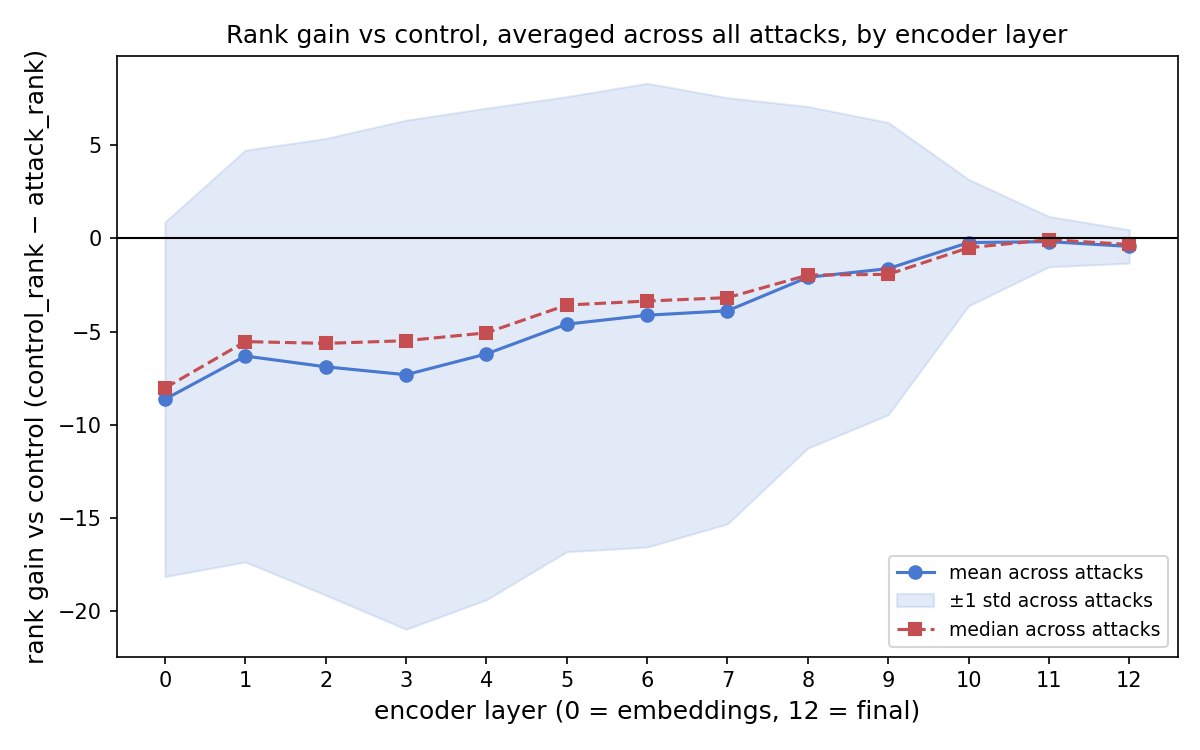
\includegraphics[width=0.75\textwidth]{outputs/attack_comparison/mean_rank_gain_trajectory.png}
  \caption{Mean and median rank\_gain\_vs\_control, averaged/medianed across
  all 226 attacks, at every one of the 13 encoder depths (the same quantity
  reported at only 5 layers in Table~\ref{tab:trajectory}). The shaded band
  is $\pm 1$ standard deviation \emph{across attacks} at each layer —
  its width is itself evidence of the token-level heterogeneity discussed
  below.}
  \label{fig:meantrajectory}
\end{figure}

\begin{figure}[H]
  \centering
  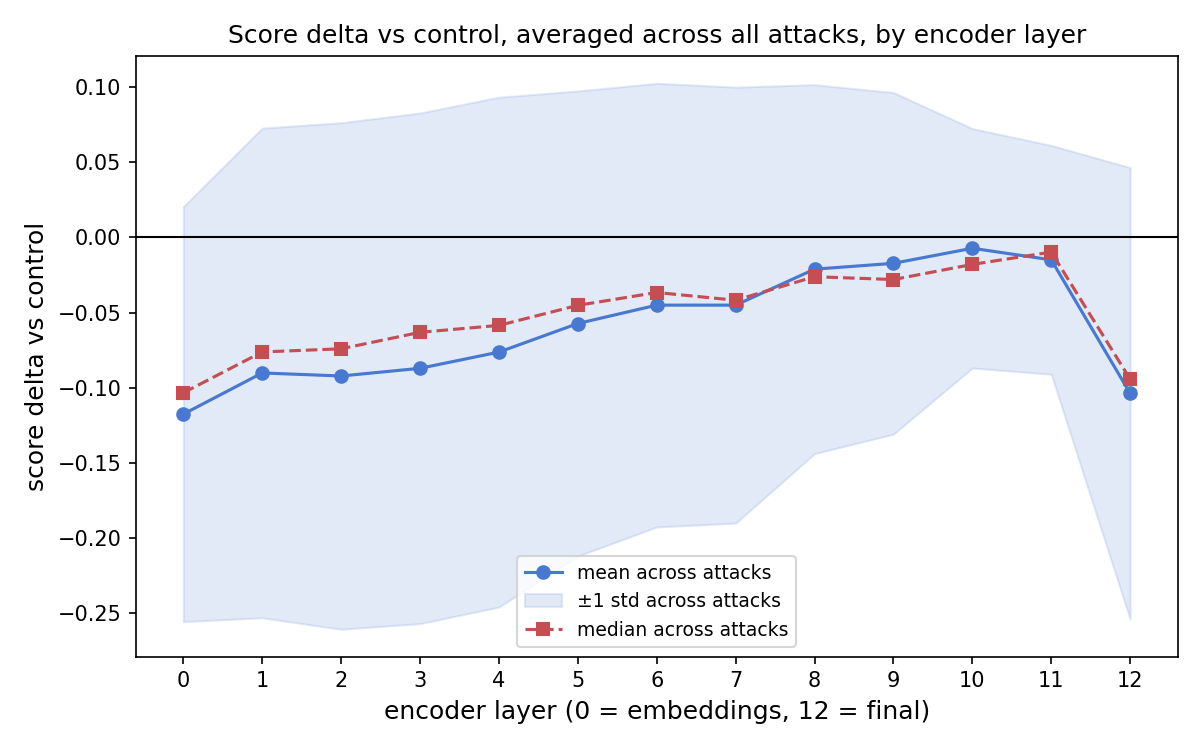
\includegraphics[width=0.75\textwidth]{outputs/attack_comparison/mean_score_delta_trajectory.png}
  \caption{Mean and median score\_delta\_vs\_control (the un-ranked, raw
  logit-difference version of the same quantity), across all 226 attacks
  and all 13 depths. Same overall shape as Figure~\ref{fig:meantrajectory}
  (monotonic climb toward zero, late-layer dip), confirming the ranking
  metric is not manufacturing a pattern absent from the underlying scores.}
  \label{fig:scoretrajectory}
\end{figure}

\begin{figure}[H]
  \centering
  
\includegraphics[width=0.55\textwidth]{outputs/attack_comparison/rank_gain_heatmap.png}
  \caption{Median rank gain vs.\ control, every attack (rows) by encoder
  layer (columns). Blue = attack hurt the target's rank at that layer; red
  = attack helped. Substantial heterogeneity: some tokens (\texttt{false},
  \texttt{falses}) are strongly blue through the middle layers; others
  (\texttt{pertinent}) are strongly red.}
  \label{fig:heatmap}
\end{figure}

\paragraph{Both mean and median tell the same story.} At the embedding
layer (0) and the earliest encoder blocks, the target's rank is, on
average, far \emph{worse} under attack than under padded control
(mean $-8.63$, i.e.\ roughly 9 positions worse out of 100) — the
un-contextualised, early representation of the attacked passage is if
anything actively misleading relative to control. This recovers steadily
and almost monotonically with depth, crossing into near-neutral territory
by layers 10--11 (mean $-0.23$/$-0.18$), as plotted continuously across all
13 depths in Figure~\ref{fig:meantrajectory} rather than only the 5 sampled
columns of Table~\ref{tab:trajectory}. \textbf{The final layer (12) is a
partial exception}: both mean ($-0.44$) and median ($-0.34$) rank gain are
measurably \emph{worse} than layers 10--11, and mean score delta jumps from
$-0.015$ (layer 11) to $-0.104$ (layer 12) — a real, reproducible dip in
the aggregate, not just one outlier attack (Section~\ref{sec:latedip}), and
visible as the small uptick at the right edge of Figure~\ref{fig:meantrajectory}
(the corresponding score-delta trajectory, same shape, is in
Figure~\ref{fig:scoretrajectory}).

\paragraph{Success rate follows an inverted-U, not a monotonic curve.} The
fraction of examples where the attack actually beats the padded control
(regardless of margin) \emph{peaks at layers 6--8} ($\approx$35\%), higher
than at either the earliest layers ($\approx$18\% at layer 0) or the final
layer ($\approx$17\% at layer 12). Read together with the rank-gain
trajectory, this suggests two different things are happening at different
depths: by mid-depth, a broad plurality of examples show \emph{some} small
positive effect; by the final layers, \emph{fewer} examples succeed, but
among the strong attacks that do, the margin is much larger — the mean is
increasingly driven by a shrinking set of big winners rather than broad
consensus.

\subsection{How much of the recovery is attack-specific?}
\label{sec:sharedrecovery}

\begin{figure}[H]
  \centering
  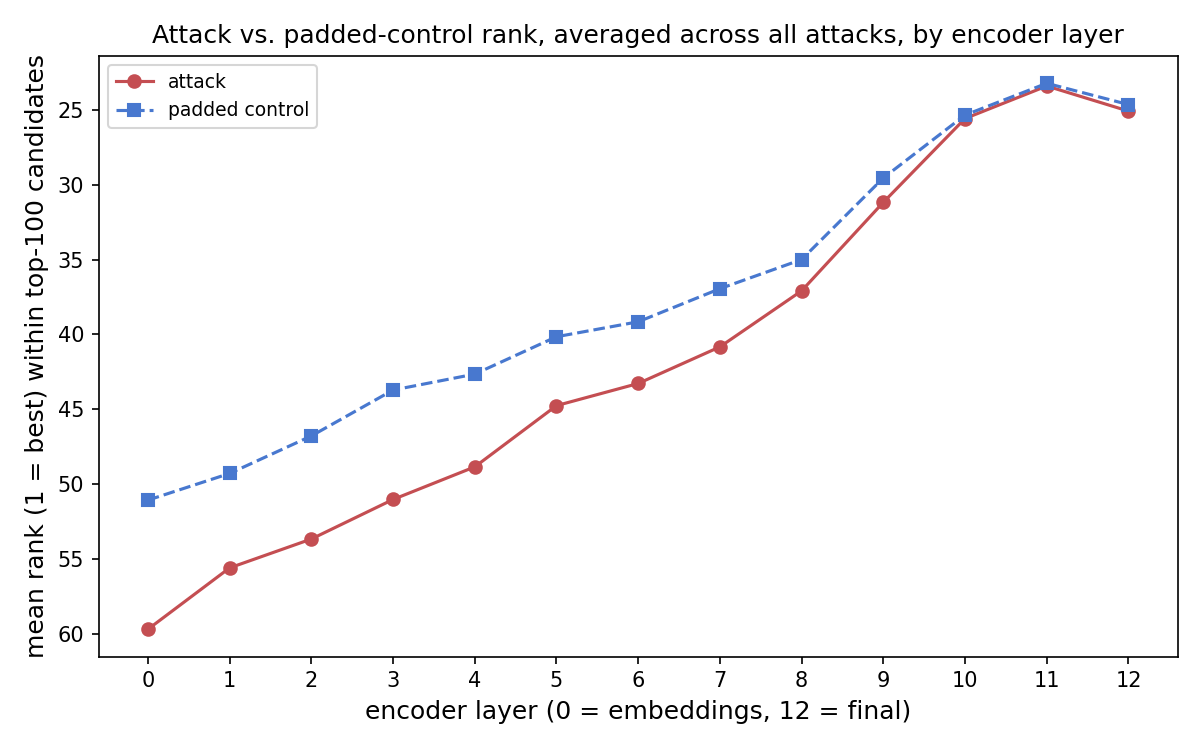
\includegraphics[width=0.75\textwidth]{outputs/attack_comparison/attack_vs_control_rank_trajectory.png}
  \caption{Mean raw rank (not rank \emph{gain}) of the \texttt{attack} and
  \texttt{padded\_control} variants separately, averaged across all 226
  attacks, at every encoder depth (y-axis inverted so rank 1, best,
  is at the top). Both variants improve from near rank 50--60 at the
  embedding layer to $\approx$23--25 by layers 10--12 — most of the
  ``recovery'' described above is shared with the control, not unique to
  the attack.}
  \label{fig:attackvscontrol}
\end{figure}

Figure~\ref{fig:meantrajectory}'s recovery curve is a \emph{difference}
(rank\_gain\_vs\_control = control\_rank $-$ attack\_rank); it is worth
asking how much of that recovery reflects the attack becoming
representationally legible versus the encoder simply becoming more
discriminative for \emph{any} input as depth increases.
Figure~\ref{fig:attackvscontrol} plots the two raw rank trajectories
separately and shows both climbing together: the padded control improves
from mean rank 51.1 (layer 0) to 23.2 (layer 11), and the attack from 59.7
to 23.4 over the same span — a $\approx$28-position improvement for
\emph{both} variants. Only the residual \emph{gap} between the two
curves — $8.6$ positions at layer 0, narrowing to $0.2$ at layer 11 before
widening slightly back to $0.4$ at layer 12 — is attributable to the
attack specifically (this gap is exactly the quantity plotted in
Figure~\ref{fig:meantrajectory}). The practical implication is that the
depth range identified here (layers 10--11) should be read as \emph{where
the attack's residual effect becomes smallest relative to a generically
more discriminative encoder}, not as the depth at which the attacked
content is first ``read'' by the model in an absolute sense — both framings
support the same layer-range conclusion, but the causal story is about a
narrowing gap, not a rank that only the attack recovers.
consensus.

\subsection{The final-layer dip, explained by best-layer distribution}
\label{sec:latedip}

\begin{figure}[H]
  \centering
  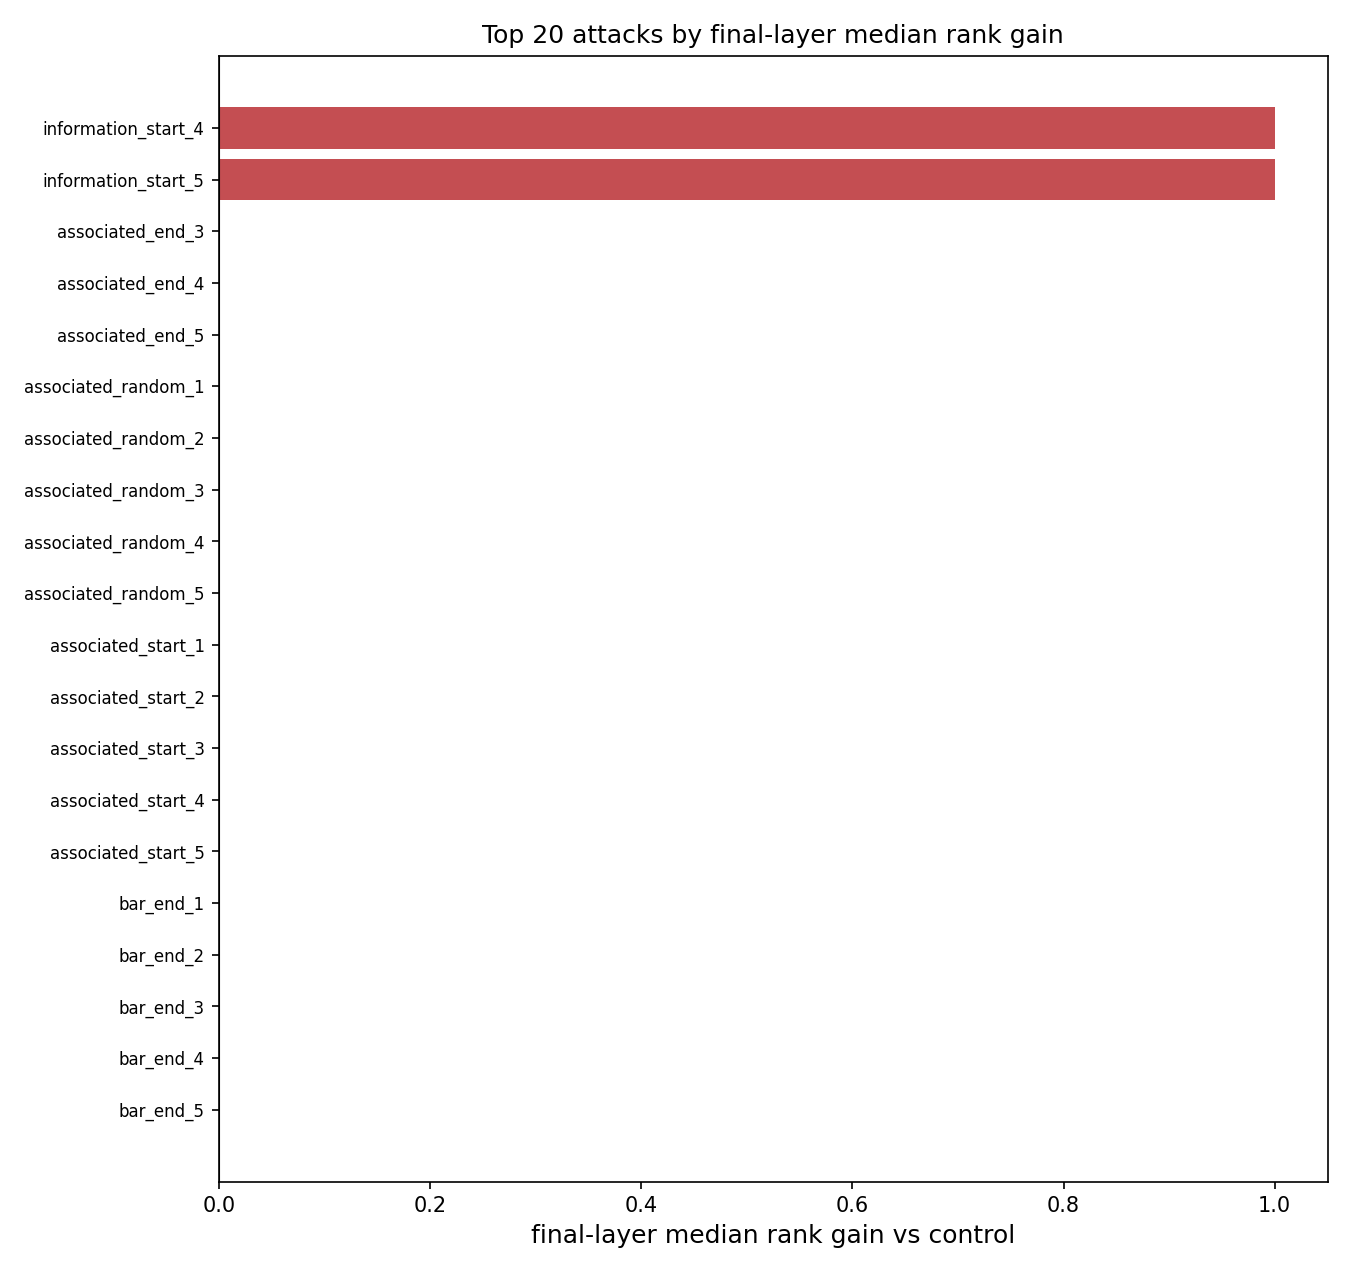
\includegraphics[width=0.9\textwidth]{outputs/attack_comparison/top_attacks_rank_gain.png}
  \caption{Top 20 attacks by final-layer mean rank gain vs.\ control.}
  \label{fig:topattacks}
\end{figure}

The layer at which each individual attack achieves its \emph{best} rank
gain is concentrated late but not exclusively so:
\textbf{layer~11 is best for 64/226 attacks (28\%) and layer~10 for 33/226
(15\%)} — the modal choice by a wide margin — but the remaining 129
attacks (57\%) peak somewhere else, including a handful (3) that peak at
layer~0. Layer~12's aggregate dip relative to layer~11 is consistent with
many individual attacks' \emph{best} layer being 10 or 11, not 12 — i.e.\
for a substantial fraction of attacks, the fully-contextualised final
representation is measurably \emph{less} favourable to the target than the
penultimate one or two layers, even though layer~12 is what ordinary
monoT5 scoring actually uses.

\subsection{Token, position, and repetition effects — most tokens do not work}

\begin{table}[H]
\centering
\caption{Mean final-layer rank gain by token, best and worst 4 of 16.}
\begin{tabular}{lr|lr}
\toprule
Best tokens & Rank gain & Worst tokens & Rank gain \\
\midrule
information & $+0.521$ & bar            & $-0.945$ \\
irrelevant  & $+0.149$ & baz            & $-1.041$ \\
relevance   & $-0.109$ & informationbaz & $-1.146$ \\
associated  & $-0.127$ & relevancy      & $-0.749$ \\
\bottomrule
\end{tabular}
\end{table}

Only \texttt{information} and \texttt{irrelevant} have a \emph{positive}
mean final-layer rank gain across all their position/repetition variants;
the other 14 of 16 tokens are net negative. That \texttt{irrelevant} —
lexically the antonym of what the attack is trying to convey — still
produces a small positive rank gain is a striking, if modest, confirmation
that monoT5's vulnerability is substantially about surface-level keyword
repetition rather than genuine semantic content: the model does not
reliably distinguish ``irrelevant: irrelevant: \ldots'' from
``relevant: relevant: \ldots'' as a ranking signal, even though the two
phrases mean opposite things.

By \textbf{position}, aggregated over all 16 tokens, \texttt{end} is the
only position with a positive mean rank gain ($+0.076$); \texttt{start}
($-0.513$) and \texttt{random} ($-0.880$) are both negative. This appears
to contradict Experiment~1's finding that \texttt{start} position was
strongest — but Experiment~1's finding was specifically about the 7
curated, generally-effective tokens (\texttt{relevant}, \texttt{information},
etc.); this broader 16-token aggregate is dominated by the majority of
tokens that are net-negative regardless of position, and among those,
\texttt{start} and \texttt{random} appear to be more actively harmful than
\texttt{end}. The two findings are not in tension once restricted to the
same token subset (Experiment~1's own within-token breakdown already shows
\texttt{information\_start\_5} as the single strongest attack in that
grid, consistent with the pattern here).

By \textbf{repetition count}, mean rank gain improves mostly monotonically
from 1 repetition ($-0.588$) to 4 ($-0.301$), with a small reversal at 5
repetitions ($-0.323$) — more stuffing generally helps, up to a point, but
the effect is not perfectly monotonic in this broader token set.

% =====================================================================
\section{Overall Interpretation and Discussion}
% =====================================================================

\begin{enumerate}
  \item \textbf{Representational readability and causal importance point to
  the same depth range, but are not the same measurement.} DecoderLens
  shows the target's rank recovering from a strongly negative early state
  to near-neutral by layers 10--11 — the same depth range where
  Experiments~1 and 3 find the causally dominant components. This is a
  useful triangulation (two independently-motivated methods agree on
  \emph{when}), but DecoderLens's success-rate inverted-U and the
  late-layer dip show a more heterogeneous, less uniformly-monotonic story
  than a causal-effect-only view would suggest. \textbf{Caveat
  (Section~\ref{sec:sharedrecovery}):} most of this recovery in absolute
  rank terms ($\approx$28 positions, embedding to layer~11) is shared
  between the attack and the padded control — only a much smaller residual
  gap ($8.6\to0.2$ positions) is attributable to the attack itself. The
  depth range should be read as where that residual gap is smallest, not
  as the depth at which the attacked content first becomes legible in an
  absolute sense.
  \item \textbf{Most keyword-stuffing attempts do not work, even by this
  lenient metric.} 14 of 16 tokens in this broader sweep have a negative
  mean final-layer rank gain. Attack success is highly specific to
  particular trigger words (chiefly ``information'' and, to a lesser
  extent, ``irrelevant''), not a generic property of repeating any
  relevance-adjacent word — consistent with, and now confirmed
  independently of, Experiment~1's score-delta-based finding that
  \texttt{bar}, \texttt{true}, \texttt{false} are weak or negative
  regardless of placement.
  \item \textbf{The antonym result is a small but genuine piece of evidence
  for surface-level (not semantic) vulnerability.} \texttt{irrelevant}
  improving rank, even slightly, is hard to explain if the model were
  robustly parsing the stuffed phrase's actual meaning.
  \item \textbf{The final layer is not always where the target looks best.}
  For a majority of individual attacks (57\%), the best-ranking encoder
  depth is \emph{not} the final layer — a finding with no direct causal
  interpretation from this experiment alone, but a natural target for a
  future DecoderLens-guided activation-patching follow-up focused on
  layers 8--11 rather than only the final block.
\end{enumerate}

% =====================================================================
\section{Limitations and Threats to Validity}
% =====================================================================

\begin{itemize}
  \item \textbf{Purely representational, not causal.} DecoderLens
  identifies \emph{when} information becomes visible to a re-read-out, not
  \emph{why} — it makes no patching or ablation claim, and should be read
  as complementary to, not a replacement for, Experiments~1/3.
  \item \textbf{Ranking against a fixed, never-recomputed BM25 candidate
  set.} All 99 other candidates are scored only once (clean); the
  candidate set's own composition is exactly what the original ECIR-24
  BM25 run produced and is not revisited here.
  \item \textbf{One incomplete attack.} \texttt{relevant\_end\_2} has
  alignment output but no scores; excluded from all aggregate statistics
  (226/227 used).
  \item \textbf{Broader, less curated attack set.} The 16-token, 226-attack
  set intentionally goes beyond the 7-token, 105-attack grid used
  elsewhere in this project, which makes cross-experiment numeric
  comparison approximate rather than exact — differences in aggregate
  trends (e.g.\ the position effect above) can reflect the different token
  mix, not a contradiction.
  \item \textbf{Single model/dataset.} Results are for monoT5-base on
  DL19, matching the rest of this project.
\end{itemize}

% =====================================================================
\section{Reproducibility}
% =====================================================================

From \texttt{monot5\_decoderlens\_rank/}, with the \texttt{advseq2seq}
conda environment:

\begin{lstlisting}
# Smoke test (1 attack, 20 candidates, 5 targets) -> outputs_smoke/
bash bash/run_all_decoderlens_attacks.sh configs/smoke.yaml --force

# Full run over all discovered attacks -> outputs/
bash bash/run_all_decoderlens_attacks.sh configs/default.yaml

# Cross-attack comparison only (fast — pure aggregation of existing per-attack CSVs)
python3 scripts/06_compare_decoderlens_attacks.py --config configs/default.yaml
\end{lstlisting}

\noindent Per-attack outputs under \texttt{outputs/attacks/\{attack\}/};
cross-attack comparison (summary CSV + 6 plots) under
\texttt{outputs/attack\_comparison/}.

% =====================================================================
\section*{Appendix: Glossary of Key Quantities}
\addcontentsline{toc}{section}{Appendix: Glossary of Key Quantities}
% =====================================================================

\begin{description}[leftmargin=1.8em,style=nextline]
  \item[DecoderLens] forcing the decoder to cross-attend to an
  \emph{intermediate} encoder layer's (final-layer-norm-applied) hidden
  states instead of the true final output; a representational, non-causal
  probe.
  \item[$\score_l$] DecoderLens score at encoder depth $l$ (0 = embeddings,
  12 = final layer, matching ordinary monoT5 scoring).
  \item[rank\_gain\_vs\_control] $\text{control\_rank} - \text{attack\_rank}$
  within the fixed top-100 BM25 candidate set; positive = attack improved
  the target's position.
  \item[success\_rate\_vs\_control] fraction of examples where
  rank\_gain\_vs\_control $>0$ (or score\_delta $>0$ for the score-based
  variant).
  \item[best\_layer\_by\_rank\_gain] the encoder depth at which one attack's
  mean rank gain is highest.
  \item[padded control / attack / original] the same three input variants
  used throughout this project (Type~B/C/A).
\end{description}

\end{document}
